\chapter{Connect Model to Libraries}
In Chapter 2, we stored the information of a higher-order linear ODE in the \verb|DifferentialModel|. This \verb|data type| preserves the relationship of the ODE, and we can transform the ODE into other forms. In Chapter 3, we discuss how to solve a system of first-order ODE numerically in four selected external libraries. However, there is a gap between the \verb|DifferentialModel| and external libraries. If we can close it, the Drasil framework can generate a program that unitize external libraries to solve a high-order ODE numerically. All external libraries cannot directly utilize \verb|DifferentialModel|, so this is the problem we will solve in this chapter. We know that most ways of solving ODEs are intended for first-order ODE, so we want to convert most higher-order ODEs to a system of first-order ODE~\citep{converthigherode}. Therefore, we first transform a higher-order linear ODE into a system of first-order ODE. Then, generating a program that contains proper interfaces for utilizing four selected external libraries. This program solves the system of first-order ODE numerically. The original higher-order linear ODE is equivalent to the system of first-order ODE we solved. Thus, by transitivity, the numerical solution for the system of first-order ODE is also the numerical solution of the higher-order ODE.

In this chapter, we will first discuss how to convert any higher-order linear ODE to a system of first-order ODE in theory. Then, we will discuss about how to enable Drasil Code Generator to generate a program that produce numerical solution for a system of first-order ODE. Lastly, we will discuss about how to automate the generating process.

\section{Higher Order to First Order}
\label{se_hightofirst}
Given a higher-order linear ODE, we can write it as Equation~\ref{eq_isohighode}. We isolate the highest derivative $y^n$ on the left-hand side and the rest of terms on the right- hand side. On the right hand side, $f (t, y, y', y'', \dots, y^{n-1})$ means a function depends on variables t, y, y', \dots, and $y^{n-1}$. The t is the independent variable, and it is often time. The y, y', \dots, and $y^{n-1}$ means the dependent variable y, the first derivative of y, and until the (n-1)th derivative.
\begin{equation} \label{eq_isohighode}
  y^n = f (t, y, y', y'', \dots, y^{n-1})
\end{equation}

Then, we start to introducing new variables, $x_{1}$, $x_{2}$, $\dots$, and $x_{n}$. The number of the newly introduced dependent variable is equal to the highest order of the ODE. The new relationship is shown below.
\begin{flalign} \label{eq_newvars}
  & x_{1} = y \\ \nonumber
  & x_{2} = y' \\ \nonumber
  & \dots \\ \nonumber
  & x_{n} = y^{n-1} 
\end{flalign}

After that, we start to differentiating $x_{1}$, $x_{2}$, $\dots$, and $x_{n}$ in Equation~\ref{eq_newvars}. This step helps us to get new relationships between each variable.
\begin{flalign} \label{eq_diffvervars}
  & x_{1}' = y' = x_{2} \\ \nonumber
  & x_{2}' = y'' = x_{3} \\ \nonumber
  & \dots \\ \nonumber
  & x_{n-1}' = y^{n-1} = x_{n}\\ \nonumber
  & x_{n}' = y^{n} = f (t, x_{1}, x_{2}, \dots, x_{n})
\end{flalign}

Since the higher-order ODE is linear ODE, $f (t, x_{1}, x_{2}, \dots, x_{n})$ is a linear function. We can rewrite $f (t, x_{1}, x_{2}, \dots, x_{n})$ as the following
\begin{equation}\label{eq_linear}
b_{0}(t) \cdot x_{1} + b_{1}(t) \cdot x_{2} + \dots + b_{n-1}(t) \cdot x_{n} + h(t)
\end{equation}
$b_{0}(t)$, $\dots$, $b_{n-1}(t)$ and $h(t)$ are constant functions.

Based on Equation~\ref{eq_diffvervars} and Equation~\ref{eq_linear}, we can we can get:
\begin{flalign} \label{eq_diffvervarslinear}
    & x_{1}' = x_{2} \\ \nonumber
    & x_{2}' = x_{3} \\ \nonumber
    & \dots \\ \nonumber
    & x_{n-1}' = x^{n}\\ \nonumber
    & x_{n}'= b_{0}(t) \cdot x_{1} + b_{1}(t) \cdot x_{2} + ... + b_{n-1}(t) \cdot x_{n} + h(t)
\end{flalign}

Then, we can rewrite Equation~\ref{eq_diffvervarslinear} in a matrix form.
\begin{equation} \label{eq_foodeexample}
	\begin{bmatrix}
		x_{1}' \\
    x_{2}' \\
    \dots  \\
    x_{n-1}' \\
    x_{n}'
	\end{bmatrix}
    = 
  \begin{bmatrix}
		0, & 1, & 0, & \dots, & 0 \\
    0, & 0, & 1, & \dots, & 0 \\
    \dots \\
    0, & 0, & 0, & \dots, & 1 \\
    b_{0}(t), & b_{1}(t), & b_{2}(t), & \dots, & b_{n-1}(t)
	\end{bmatrix}
    \cdot
  \begin{bmatrix}
		x_{1} \\
    x_{2} \\
    \dots  \\
    x_{n-1} \\
    x_{n}
	\end{bmatrix}
    + 
  \begin{bmatrix}
    0 \\
    0 \\
    \dots  \\
    0 \\
    h(t)
	\end{bmatrix}
\end{equation}

Lastly, we abstract Equation~\ref{eq_foodeexample} into a general form, Equation~\ref{eq_foode}. 
\begin{equation} \label{eq_foode}
    \boldsymbol{X}' = \boldsymbol{AX} + \boldsymbol{c}
\end{equation}
The \textbf{A} is a coefficient matrix, and \textbf{c} is a constant vector. The \textbf{X} is the unknown vector that contains functions of the independent variable, often time. The \textbf{X}' is a vector that consists of first derivatives of functions of \textbf{X}.

% Once we complete the transformation, we get a system of first-order ODE in the shape of Equation~\ref{eq_foode}. We encode it in Drasil and pass it to Drasil Code Generator. In the \href{https://jacquescarette.github.io/Drasil/examples/pdcontroller/SRS/srs/PDController_SRS.html#Sec:IMs}{PDContoller case study}, we convert Example~\ref{eq_odeexmaple} to Example~\ref{ex_firstorderode}. Then, we generate a program to solve Example~\ref{ex_firstorderode} numerically. By transitivity, the numerical solution is valid for Example~\ref{eq_odeexmaple} as well.

\section{Connect Explicit Equations to Libraries}
\label{se_connecteetolib}

In previous research conducted by Brooks, we wrote the ODE in a text-based form and stored them in a general data pool. Although, the Drasil printer can print a text-based ODE in the SRS, the Drasil Code Generator cannot utilize the text-based ODE. Therefore, we manually create a \verb|data type|, called \verb|ODEInfo|, to make study cases work. We extract useful information from the original ODE and construct \verb|ODEInfo| for Dasil Code Generator. The Drasil Code Generator utilized \verb|ODEInfo| to generate a program which produce a numerical solution. We can find details on how to generate a program which solve the ODE numerically in Brooks's thesis~\citep{brooks}. However, the previous research only completed generating a program for a first-order ODE. Since it is a first-order ODE, we only provide an initial value. For a higher-order ODE, the current setting of \verb|ODEInfo| does not hold all information we need to solve a ODE. Therefore, to enable Drasil Code Generator generating problem for higher-order ODE, the \verb|ODEInfo| need to store multiple initial values. For example, we can convert a fourth-order ODE into a system of first-order ODE. To solve the system ODE as an IVP, we need four initial values. Then, the Drasil Code Generator must adapt to handle multiple initial values.

In Code~\ref{code_odeinfointial}, we change the \verb|data type| of \verb|initVal| from a \verb|CodeExpr| to a list of \verb|CodeExpr|. This change allows Drasil users store multiple initial values in a list. Before this change, we can only store one initial value. 

\begin{listing}[ht]
\begin{haskell1}
-- Old 
data ODEInfo = ODEInfo {
  ...
  initVal :: CodeExpr
  ...
}

-- New 
data ODEInfo = ODEInfo {
  ...
  initVal :: [CodeExpr],
  ...
}
\end{haskell1}
\captionof{listing}{Source code for initial values}
\label{code_odeinfointial}
\end{listing}

\begin{listing}[ht]
\begin{haskell1}
-- Old 
initVal info

-- New 
matrix[initVal info]  
\end{haskell1}
\captionof{listing}{Source code for initial values in Code Generator}
\label{code_odeinfointialcodegen}
\end{listing}

We also have to ensure Drasil Code Generator can utilize the new \verb|data type| \verb|[CodeExpr]|. Previously, Drasil Code Generator only handling the \verb|initVal| as \verb|CodeEXpr|. Now the \verb|initVal| becomes \verb|[CodeEXpr]|. In the Drasil framework, we handling a list of \verb|data type| by \href{https://jacquescarette.github.io/Drasil/docs/drasil-code-base-0.1.9.0/Language-Drasil-CodeExpr.html#v:matrix}{matrix}. The code \verb|initVal info| is just retrieves the \verb|initVal| from an \verb|ODEInfo| data type. In Code~\ref{code_odeinfointialcodegen}, the \verb|matrix| can wrap a \verb|[CodeEXpr]| into a \verb|CodeEXpr|. This change effects generated code. In Python Scipe Code~\ref{code_pythonintial}, it initialize the initial value with a list rather than one entity. The same thing happens in C\# OSLO Code~\ref{code_csharpintial}. It initializes a list rather than one object. In Java and C\texttt{++}, the backend code already handles the initial value as a list, so there is no change in artifact for those two languages. 

\begin{listing}[ht]
\begin{python1}
# Old 
  r.set_initial_value(T_init, 0.0)
  T_W = [T_init]

# New 
  r.set_initial_value([T_init], 0.0)
  T_W = [[T_init][0]] # Initial values are also a part of the numerical solution, so we have to add the proper initial value to the list.
\end{python1}
\captionof{listing}{Source code for initial values in Python}
\label{code_pythonintial}
\end{listing}

\begin{listing}[ht]
\begin{csharp1}
// Old 
Vector initv = new Vector(T_init);

// New 
Vector initv = new Vector(new double[] {T_init});
\end{csharp1}
\captionof{listing}{Source code for initial values in C\#}
\label{code_csharpintial}
\end{listing}

Allowing multiple initial values unlocks the potential for Drasil to generate a program that produce numerical solution for a system of first-order ODE. Since every higher-order linear ODE has its equivalent system of first-order ODE, the solution for the system of first-order ODE is also the solution for the higher-order ODE. The same thing happens on non-linear higher-order ODE. If we could transform a higher-order non-linear ODE to a system of first-order ODE, we can solve it through four selected external libraries. 

Despite the \href{https://jacquescarette.github.io/Drasil/examples/dblpendulum/SRS/srs/DblPendulum_SRS.html#Sec:IMs}{Double Pendulum case study} containing a higher-order non-linear ODE, the Drasil framework can now generate a program to solve it numerically. In the double pendulum case study, we eventually want to solve Equation~\ref{eq_dblpenhigh}. There are two second-order ODEs in one system. To solve this system of ODE, we convert them into a system of first-order ODE. The transformation follows the methodology we discussed in Section~\ref{se_hightofirst}. We can convert Equation~\ref{eq_dblpenhigh} into Equation~\ref{eq_dblpenfirst}. Once the transformation is complete, we can encode Equation~\ref{eq_dblpenfirst} and pass it to the Drasil Code Generator. However, we cannot show Equation~\ref{eq_dblpenfirst} in the shape of Equation~\ref{eq_foode} (\textbf{X'} = \textbf{AX} + \textbf{c}) because the ODE is not a linear ODE.

\begin{flalign} \label{eq_dblpenhigh}
& \theta_{1}'' = \frac{-g(2m_{1}+m_{2})\sin \theta_{1}-m_{2}g\sin (\theta_{1}-2\theta_{2})-2\sin (\theta_{1}-\theta_{2})m_{2}({\theta_{2}'}^2L_{2}+{\theta_{1}'}^2L_{1}\cos (\theta_{1}-\theta_{2}))}{L_{1}(2m_{1}+m_{2}-m_{2}\cos (2\theta_{1}-2\theta_{2}))} \\ \nonumber
& \theta_{2}'' = \frac{2\sin (\theta_{1}-\theta_{2})({\theta_{1}'}^2L_{1}(m_{1}+m_{2})+g(m_{1}+m_{2})\cos \theta_{1} + {\theta_{2}'}^2L_{2}m_{2}\cos (\theta_{1}-\theta_{2}))}{L_{2}(2m_{1}+m_{2}-m_{2}\cos (2\theta_{1}-2\theta_{2}))}
\end{flalign}

\begin{flalign} \label{eq_dblpenfirst}
  & \theta_{1}' = \omega_{1} \\ \nonumber
  & \theta_{2}' = \omega_{2} \\ \nonumber
  & \omega_{1}' = \frac{-g(2m_{1}+m_{2})\sin \theta_{1}-m_{2}g\sin (\theta_{1}-2\theta_{2})-2\sin (\theta_{1}-\theta_{2})m_{2}({\omega{2}}^2L_{2}+{\omega{1}}^2L_{1}\cos (\theta_{1}-\theta_{2}))}{L_{1}(2m_{1}+m_{2}-m_{2}\cos (2\theta_{1}-2\theta_{2}))} \\ \nonumber
  & \omega_{2}' = \frac{2\sin (\theta_{1}-\theta_{2})({\omega_{1}}^2L_{1}(m_{1}+m_{2})+g(m_{1}+m_{2})\cos \theta_{1} + {\omega_{2}}^2L_{2}m_{2}\cos (\theta_{1}-\theta_{2}))}{L_{2}(2m_{1}+m_{2}-m_{2}\cos (2\theta_{1}-2\theta_{2}))}
\end{flalign}

Figure~\ref{fig_dblpen} demonstrates how a double pendulum example in a lab environment. The full details of the double pendulum's SRS in \href{https://jacquescarette.github.io/Drasil/examples/dblpendulum/SRS/srs/DblPendulum_SRS.html}{Drasil website}. Table~\ref{tab_dblpendes} lists the all variable means in the example.
\begin{figure}[ht]
  \centering
  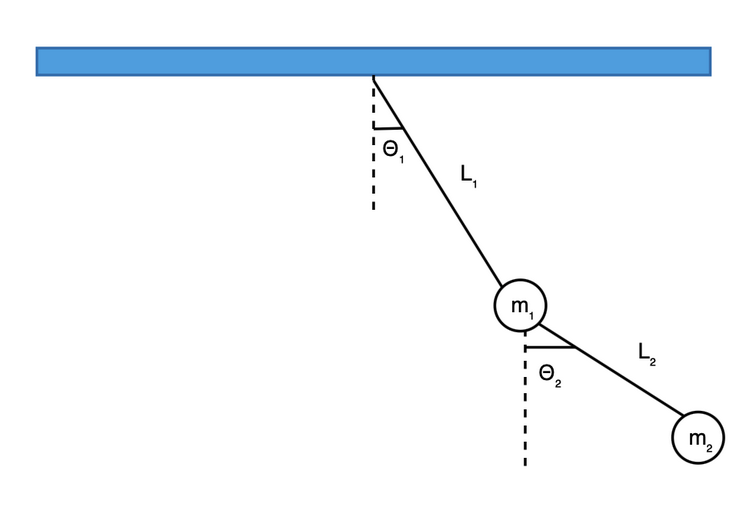
\includegraphics[width=0.6\textwidth]{figures/DblPendulum.png}
  \caption{Double Pendulum Demonstration}
  \label{fig_dblpen}
\end{figure}

\begin{table}[ht]
	\begin{tabular}{ p{0.2\textwidth} p{0.7\textwidth} }
		\textbf{Name} & \textbf{Description} \\
		\toprule
		\verb|m₁| & The mass of the first object\\
    \verb|m₂| & The mass of the second object\\
		\verb|L₁| & The length of the first rod\\
		\verb|L₂| & The length of the second rod\\
		\verb|g| & gravity\\
		\verb|θ₁| & The angle of the first rod\\
		\verb|θ₂| & The angle of the second rod\\
		\verb|ω₁| & The angular velocity of the first object\\
		\verb|ω₂| & The angular velocity of the second object\\
		\bottomrule	
	\end{tabular}	
	\caption{Variables in Double Pendulum Example}	
	\label{tab_dblpendes}
\end{table}

Now we have Equation~\ref{eq_dblpenfirst}, we can encode it in the Drasil. In Code~\ref{code_encodedblpend}, it shows the example of how we encode Equation~\ref{eq_dblpenfirst} in the Drasil. 
\begin{listing}[ht]
\begin{haskell1}
dblPenODEInfo :: ODEInfo
dblPenODEInfo = odeInfo
...
[3*π/7, 0, 3*π/4, 0]
[ ω₁,
  -g(2m₁ + m₂)sin θ₁ - m₂gsin (θ₁ - 2θ₂) - 2sin (θ₁ - θ₂)m₂(ω₂²L₂ + ω₁²L₁cos (θ₁ - θ₂)) / L₁(2m₁ + m₂ -m₂cos (2θ₁ - 2θ₂)),
  ω₂,
  2sin (θ₁ - θ₂)(ω₁²L₁(m₁ + m₂ ) + g(m₁ + m₂ )cos θ₁ + ω₂²L₂m₂cos (θ₁ - θ₂ )) / L₂(2m₁ + m₂ -m₂cos (2θ₁ - 2θ₂))
]
...
\end{haskell1}
\captionof{listing}{Source code for encoding double pendulum}
\label{code_encodedblpend}
\end{listing}

Once the \verb|dblPenODEInfo| is ready, we will pass it to the Drasil Code generator. It will generate programs solve Double Pendulum in four languages. The details of generated code for double pendulum will show in Appendix A ("Should I list all generated code in Appendix, it looks ugly"). However, the Double Pendulum case study unable to utilize any function introduced in the next section because it was designed for a linear ODE.

The limitation of manually creating \verb|ODEInfo| is that we will write the ODE twice. In this case, we encode both Equation~\ref{eq_dblpenhigh} and Equation~\ref{eq_dblpenfirst} in Drasil. They both demonstrate the phenomena of double pendulum, and exist in an isomorphic ODE type. In the next section, we would like to discuss how to automate the transformation from a higher-order ODE to a system of first-order ODE.

\section{Generate Explicit Equations}
Manually creating explicit equations is not ideal because it requires human interference and propagates duplicate information. We want to design the Drasil framework as fully automatically as possible, so we want to remove human interference. Therefore, an ideal solution is to encode the ODE in a flexible data structure. Then, we extract information from this structure and generate a form of ODE which selected external libraries can utilize. Creating the \verb|DifferentialModel| data structure satisfies the need of this idea. We can restructure an ODE base on the information from \verb|DifferentialModel|. This research's scope only covers generating explicit equations for a single higher-order ODE. In the future, we are looking to generate explicit equations for a system of higher-order ODE.

Once we encode the ODE in \verb|DifferentialModel|, we want to restructure its equivalent system of first-order ODE in the shape of Equation~\ref{eq_foode}. For the convenience of implementation, we shuffle the data around in Equation~\ref{eq_foodeexample}. We reversed the order of \textbf{X} to $x_{n}$, $\dots$, $x_{1}$. The coefficient matrix \textbf{A} also changed, but \textbf{X'} and \textbf{c} remain unchanged.

\begin{equation} \label{eq_foodeexamplecolor}
	\begin{bmatrix}
		\highlight{yellow}{x_{1}'} \\
    \highlight{yellow}{\dots} \\
    \highlight{yellow}{x_{n-2}'} \\
    \highlight{yellow}{x_{n-1}'} \\
    \highlight{yellow}{x_{n}'}
	\end{bmatrix}
    = 
  \begin{bmatrix}
		\highlight{orange}{0}, & \highlight{orange}{0}, & \highlight{orange}{\dots}, & \highlight{orange}{1}, & \highlight{orange}{0} \\
    \highlight{orange}{\dots} \\
    \highlight{orange}{0}, & \highlight{orange}{1}, & \highlight{orange}{\dots}, & \highlight{orange}{0}, & \highlight{orange}{0} \\
    \highlight{orange}{1}, & \highlight{orange}{0}, & \highlight{orange}{\dots}, & \highlight{orange}{0}, & \highlight{orange}{0} \\
    \highlight{cyan}{b_{n-1}(t)}, & \highlight{cyan}{b_{n-2}(t)}, & \highlight{cyan}{\dots}, & \highlight{cyan}{b_{1}(t)}, & \highlight{cyan}{b_{0}(t)}
	\end{bmatrix}
    \cdot
  \begin{bmatrix}
    \highlight{yellow}{x_{n}} \\
    \highlight{yellow}{\dots} \\
    \highlight{yellow}{x_{3}} \\
		\highlight{yellow}{x_{2}} \\
    \highlight{yellow}{x_{1}}
	\end{bmatrix}
    + 
  \begin{bmatrix}
    \highlight{lightgray}{0} \\
    \highlight{lightgray}{0} \\
    \highlight{lightgray}{\dots} \\
    \highlight{lightgray}{0} \\
    \highlight{red}{h(t)}
	\end{bmatrix}
\end{equation}

Since Equation~\ref{eq_foodeexamplecolor} is an expansion of Equation~\ref{eq_foode}, we will use symbols in both equations to explain how to generate Equation~\ref{eq_foodeexamplecolor}. We highlighted \textbf{X'} and \textbf{X} in yellow colour in Equation~\ref{eq_foodeexamplecolor}. The number of elements in \textbf{X'} and \textbf{X} depends on how many new dependent variables introduces. If the higher-order ODE is second-order, we will introduce two new dependent variables. If the higher-order ODE is nth-order, we will introduce n new dependent variables. For \textbf{X'}, knowing it is n-th order ODE, we parameterize $x'$ from 1 to n. For \textbf{X}, knowing it is n-th order ODE, we parameterize $x$ from n to 1.

% In Chapter, we create \verb|DifferentialModel| to represent the ODE in matrix form. 

% Fix-me DE model need to remove the highest order. Once we isolation the highest order on the left side, there will be no highest order in right side
% Fix-me Code implementation has highest order on the top, data will shuffle around and looks different than report

We highlighted the n$\times$n coefficient matrix \textbf{A} in orange and blue colour in Equation~\ref{eq_foodeexamplecolor}. The orange part is an matrix looks like an identity matrix. For the lowest higher-order ODE second-order, the orange part is [1, 0]. Equation~\ref{eq_foodeexamplecolortwo} shows a completed transformation for a second-order ODE.
\begin{equation} \label{eq_foodeexamplecolortwo}
	\begin{bmatrix}
		{x_{1}'} \\
    {x_{2}'} 
	\end{bmatrix}
    = 
  \begin{bmatrix}
		\highlight{orange}{1}, & \highlight{orange}{0} \\
    {b_{1}(t)}, & {b_{0}(t)}
	\end{bmatrix}
    \cdot
  \begin{bmatrix}
		{x_{2}} \\
    {x_{1}} 
	\end{bmatrix}
    + 
  \begin{bmatrix}
    {0} \\
    {h(t)}
	\end{bmatrix}
\end{equation}

If it is a fourth-order ODE, the \textbf{A} will be an n$\times$n matrix. Equation~\ref{eq_foodeexamplecolorfour} shows a completed transformation for a fourth-order ODE.
\begin{equation} \label{eq_foodeexamplecolorfour}
	\begin{bmatrix}
		{x_{1}'} \\
    {x_{2}'} \\
    {x_{3}'} \\
    {x_{4}'}
	\end{bmatrix}
    = 
  \begin{bmatrix}
		\highlight{orange}{0}, & \highlight{orange}{0}, & \highlight{orange}{1}, & \highlight{orange}{0} \\
    \highlight{orange}{0}, & \highlight{orange}{1}, & \highlight{orange}{0}, & \highlight{orange}{0} \\
    \highlight{orange}{1}, & \highlight{orange}{0}, & \highlight{orange}{0}, & \highlight{orange}{0} \\
    {b_{3}(t)}, & {b_{2}(t)}, & {b_{1}(t)}, & {b_{0}(t)}
	\end{bmatrix}
    \cdot
  \begin{bmatrix}
		{x_{4}} \\
    {x_{3}} \\
    {x_{2}} \\
    {x_{1}}
	\end{bmatrix}
    + 
  \begin{bmatrix}
    {0} \\
    {0} \\
    {0} \\
    {h(t)}
	\end{bmatrix}
\end{equation}

The orange part starts at (n-1)th row with $[1, 0, \dots]$. If there is a second row, we add $[0, 1, \dots]$ before the start row and so on. We observe there is a pattern for the orange part, so that we can generate it. In Code~\ref{code_createidentity}, \verb|constIdentityRowVect| and \verb|addIdentityValue| are responsible for each row in the orange part. We first create a row containing a list of 0. Then, we replace one of 0s to 1. The \verb|addIdentityCoeffs| run through a recursion to create a \verb|[[Expr]]| that responsible to orange part.

\begin{listing}[ht]
\begin{haskell1}
-- | Add Identity Matrix to Coefficients
-- | len is the length of the identity row,
-- | index is the location of identity value (start with 0)
addIdentityCoeffs :: [[Expr]] -> Int -> Int -> [[Expr]]
addIdentityCoeffs es len index
  | len == index + 1 = es
  | otherwise = addIdentityCoeffs (constIdentityRowVect len index : es) len (index + 1)

-- | Construct an identity row vector.
constIdentityRowVect :: Int -> Int -> [Expr]
constIdentityRowVect len index = addIdentityValue index $ replicate len $ exactDbl 0

-- | Recreate the identity row vector with identity value 
addIdentityValue :: Int -> [Expr] -> [Expr]
addIdentityValue n es = fst splits ++ [exactDbl 1] ++ tail (snd splits)
  where splits = splitAt n es
\end{haskell1}
\captionof{listing}{Source code for creating identity matrix(highlighted in orange)}
\label{code_createidentity}
\end{listing}

We highlighted the constant vector \textbf{c} in gray and red colour in Equation~\ref{eq_foodeexamplecolor}. The vector \textbf{c} has the length of n. The last element of the constant vector \textbf{c} will be h(t), and anything above h(t) will be zeros. In Code~\ref{code_createconstant}, in \verb|addIdentityConsts|, given the expression of h(t) and the order number of the ODE, we add (n-1) 0s above the h(t). 

\begin{listing}[ht]
\begin{haskell1}
-- | Add Identity Matrix to Constants
-- | len is the size of new constant vector
addIdentityConsts :: [Expr] -> Int -> [Expr]
addIdentityConsts expr len = replicate (len - 1) (exactDbl 0) ++ expr
\end{haskell1}
\captionof{listing}{Source code for creating constant matrix \textbf{c}}
\label{code_createconstant}
\end{listing}

The blue and red parts in Equation~\ref{eq_foodeexamplecolor} can be determined by Equation~\ref{eq_linearDE}. The \verb|DifferentialModel| preserves the relationship for Equation~\ref{eq_linearDE}, but it does not isolate the highest order to the left-hand side. To isolate the highest order, we have to shuffle terms between the left-hand side and right-hand side. The following is Equation~\ref{eq_linearDE}. 
\begin{equation}
	a_n(t) \cdot y^n(t) + a_{n-1}(t) \cdot y^{n-1}(t) + \dots + a_1(t) \cdot y'(t) + a_0(t) \cdot y(t) = h(t) \nonumber
\end{equation}
Firstly, we move every term from left to right, except the highest order term. 
\begin{equation}
	a_n(t) \cdot y^n(t)  = -a_{n-1}(t) \cdot y^{n-1}(t) + \dots + -a_1(t) \cdot y'(t) + -a_0(t) \cdot y(t) + h(t) \nonumber
\end{equation}
Secondly, we cancel out the coefficient, $a_n(t)$.
\begin{equation}
	y^n(t)  = \frac{-a_{n-1}(t) \cdot y^{n-1}(t) + \dots + -a_1(t) \cdot y'(t) + -a_0(t) \cdot y(t) + h(t)}{a_n(t)} \nonumber
\end{equation}
Then, this can be written in a matrix form
\begin{equation} 
  \begin{bmatrix}
		y^n(t)
	\end{bmatrix}
  = 
	\begin{bmatrix}
		-\frac{a_{n-1}(t)}{a_n(t)}, \dots, & -\frac{a_{1}(t)}{a_n(t)} & -\frac{a_{0}(t)}{a_n(t)}
	\end{bmatrix}
	\cdot
	\begin{bmatrix}
		y^{n-1}(t) \\
		\dots \\
    y'(t) \\
		y(t)  
	\end{bmatrix}
	+
	\begin{bmatrix}
		\frac{h(t)}{a_n(t)}
	\end{bmatrix}
  \nonumber
\end{equation}
Since $x_{n}'$ = $y_{n}$ (Equation~\ref{eq_diffvervars}), we can replace $y_{n}$ with $x_{n}'$. Based on Equation~\ref{eq_newvars}, we replace all derivatives of y(t) with $x_{n}$, \dots, $x_{1}$.

\begin{equation}
  \begin{bmatrix}
		x_{n}'
	\end{bmatrix}
  = 
	\begin{bmatrix}
		-\frac{a_{n-1}(t)}{a_n(t)}, \dots, & -\frac{a_{1}(t)}{a_n(t)} & -\frac{a_{0}(t)}{a_n(t)}
	\end{bmatrix}
	\cdot
	\begin{bmatrix}
		x_{n} \\
		\dots \\
    x_{2} \\
		x_{1}  
	\end{bmatrix}
	+
	\begin{bmatrix}
		\frac{h(t)}{a_n(t)}
	\end{bmatrix}
  \nonumber
\end{equation}
Lastly, we replacing new variables in Equation~\ref{eq_foodeexamplecolor}, we can get a new matrix.
\begin{equation}\label{eq_foodeexampledetail}
	\begin{bmatrix}
		\highlight{yellow}{x_{1}'} \\
    \highlight{yellow}{\dots} \\
    \highlight{yellow}{x_{n-2}'} \\
    \highlight{yellow}{x_{n-1}'} \\
    \highlight{yellow}{x_{n}'}
	\end{bmatrix}
    = 
  \begin{bmatrix}
		\highlight{orange}{0}, & \highlight{orange}{0}, & \highlight{orange}{\dots}, & \highlight{orange}{1}, & \highlight{orange}{0} \\
    \highlight{orange}{\dots} \\
    \highlight{orange}{0}, & \highlight{orange}{1}, & \highlight{orange}{\dots}, & \highlight{orange}{0}, & \highlight{orange}{0} \\
    \highlight{orange}{1}, & \highlight{orange}{0}, & \highlight{orange}{\dots}, & \highlight{orange}{0}, & \highlight{orange}{0} \\
    \highlight{cyan}{-\frac{a_{n-1}(t)}{a_n(t)}}, & \highlight{cyan}{-\frac{a_{n-2}(t)}{a_n(t)}}, & \highlight{cyan}{\dots}, & \highlight{cyan}{-\frac{a_{1}(t)}{a_n(t)}}, & \highlight{cyan}{-\frac{a_{0}(t)}{a_n(t)}}
	\end{bmatrix}
    \cdot
  \begin{bmatrix}
    \highlight{yellow}{x_{n}} \\
    \highlight{yellow}{\dots} \\
    \highlight{yellow}{x_{3}} \\
		\highlight{yellow}{x_{2}} \\
    \highlight{yellow}{x_{1}}
	\end{bmatrix}
    + 
  \begin{bmatrix}
    \highlight{lightgray}{0} \\
    \highlight{lightgray}{0} \\
    \highlight{lightgray}{\dots} \\
    \highlight{lightgray}{0} \\
    \highlight{red}{\frac{h(t)}{a_n(t)}}
	\end{bmatrix}
\end{equation}

Here is the implementation for creating Equation~\ref{eq_foodeexampledetail} in Drasil. In Code~\ref{code_isohighode}, we remove the highest order because we want to isolate the highest order to the left-hand side.
\begin{listing}[ht]
\begin{haskell1}
-- | Delete the highest order
transUnknowns :: [Unknown] -> [Unknown]
transUnknowns = tail
\end{haskell1}
\captionof{listing}{Source code for isolating the highest order}
\label{code_isohighode}
\end{listing}

In Code~\ref{code_cancelcoe}, the \verb|transCoefficients| cancel out the coefficient, $a_n(t)$, in highlighted blue. The \verb|divideCosntants| cancels out the coefficient in red highlighted.
\begin{listing}[ht]
\begin{haskell1}
-- | Cancel the leading coefficient of the highest order in the coefficient matrix
transCoefficients :: [Expr] -> [Expr]
transCoefficients es
  | head es == exactDbl 1 = mapNeg $ tail es
  | otherwise = mapNeg $ tail $ map ($/ head es) es
    where mapNeg = map (\x -> if x == exactDbl 0 then exactDbl 0 else neg x)

-- | divide the leading coefficient of the highest order in constant
divideCosntants :: Expr -> Expr -> Expr
divideCosntants a b
  | b == exactDbl 0 = error "Divisor can't be zero"
  | b == exactDbl 1 = a
  | otherwise       = a $/ b
\end{haskell1}
\captionof{listing}{Source code for canceling the coefficient from the highest order}
\label{code_cancelcoe}
\end{listing}

In Code~\ref{code_odesolverformat}, we create a new \verb|data type| called \verb|ODESolverFormat|. The \verb|ODESolverFormat| contains information for the system of first-order ODE. The \verb|coeffVects|, \verb|unknownVect|, and \verb|constantVect| are responsible for \textbf{A}, \textbf{X}, and \textbf{c} in Equation~\ref{eq_foode} (\textbf{X'} = \textbf{AX} + \textbf{c}). The \verb|makeAODESolverFormat| is a smart constructor to create an \verb|ODESolverFormat| by giving a \verb|DifferentialModel|.

\begin{listing}[ht]
\begin{haskell1}
-- Acceptable format for ODE solvers
-- X' = AX + c
-- coeffVects is A - coefficient matrix with identity matrix
-- unknownVect is X - unknown column vector after reduce the highest order
-- constantVect is c - constant column vector with identity matrix, 
-- X' is a column vector of first-order unknowns
data ODESolverFormat = X'{
  coeffVects :: [[Expr]],
  unknownVect :: [Integer],
  constantVect :: [Expr]
}

-- | Construct an ODESolverFormat for solving the ODE.
makeAODESolverFormat :: DifferentialModel -> ODESolverFormat
makeAODESolverFormat dm = X' transEs transUnks transConsts
  where transUnks = transUnknowns $ dm ^. unknowns
        transEs = addIdentityCoeffs [transCoefficients $ head (dm ^. coefficients)] (length transUnks) 0
        transConsts = addIdentityConsts [head (dm ^. dmConstants) `divideCosntants` head (head (dm ^. coefficients))] (length transUnks)
\end{haskell1}
\captionof{listing}{Source code for generating Equation~\ref{eq_foode}, \textbf{X'} = \textbf{AX} + \textbf{c}}
\label{code_odesolverformat}
\end{listing}

In Chapter 3, we mentioned we would solve the ODE as an IVP. In Code~\ref{code_ivpinfo}, we create \verb|InitialValueProblem| to store IVP-related information, includes intial time, final time and intival values.
\begin{listing}[ht]
\begin{haskell1}
-- Information for solving an initial value problem
data InitialValueProblem = IVP{
  initTime :: Expr, -- inital time
  finalTime :: Expr, -- end time
  initValues :: [Expr] -- intial values
}
\end{haskell1}
\captionof{listing}{Source code for IVP infomation}
\label{code_ivpinfo}
\end{listing}

Lastly, in Code~\ref{code_generateodeinfo}, we create a new smart construct to generate the \verb|ODEInfo| automatically. In \verb|odeInfo'|, the first parameter is \verb|[CodeVarChunk]|. There will likely be other variables in the ODE. The \verb|[CodeVarChunk]| contains variables other than the dependent and independent variables. The \href{https://jacquescarette.github.io/Drasil/docs/full/drasil-code-0.1.9.0/Language-Drasil-Data-ODEInfo.html#t:ODEOptions}{ODEOptions} is instructing external libraries on how to solve the ODE. The \verb|DifferentialModel| contains core information for the higher-order ODE. Last, \verb|InitialValueProblem| contains information for solving the ODE numerically. The \verb|createFinalExpr| creates multiple expressions in a list. Those expressions were created based on information on the system of first-order ODE. The \verb|formEquations| take parameters the coefficient matrix \textbf{A} (\verb|[[Expr]]|), the unknown vector \textbf{X}(\verb|[Unknown]|), and the constant vector(\verb|[Expr]|). Then, we form responsible expressions. The first row of \textbf{A} cross product the \textbf{X}, then we add all terms together with a responsible constant term. In the second row of \textbf{A}, we do the same thing. The \verb|formEquations| will output a list of expressions equivalent to Equation~\ref{eq_diffvervarslinear}. Once the explicit equation for the higher-order ODE is created, we can pass it to Drasil Code Generator.

\begin{listing}[ht]
\begin{haskell1}
odeInfo' :: [CodeVarChunk] -> ODEOptions -> DifferentialModel -> InitialValueProblem -> ODEInfo
odeInfo' ovs opt dm ivp = ODEInfo 
  (quantvar $ _indepVar dm) 
  (quantvar $ _depVar dm) 
  ovs 
  (expr $ initTime ivp)
  (expr $ finalTime ivp)
  (map expr $ initValues ivp)
  (createFinalExpr dm)
  opt

createFinalExpr :: DifferentialModel -> [CodeExpr]
createFinalExpr dm = map expr $ formEquations (coeffVects ode) (unknownVect ode) (constantVect ode) (_depVar dm)
  where ode = makeAODESolverFormat dm

formEquations :: [[Expr]] -> [Unknown] -> [Expr] -> ConstrConcept-> [Expr]
formEquations [] _ _ _ = []
formEquations _ [] _ _ = []
formEquations _ _ [] _ = []
formEquations (ex:exs) unks (y:ys) depVa =
  (if y == exactDbl 0 then finalExpr else finalExpr `addRe` y) : formEquations exs unks ys depVa
  where indexUnks = map (idx (sy depVa) . int) unks -- create X
        filteredExprs = filter (\x -> fst x /= exactDbl 0) (zip ex indexUnks) -- remove zero coefficients
        termExprs = map (uncurry mulRe) filteredExprs -- multiple coefficient with depend variables
        finalExpr = foldl1 addRe termExprs -- add terms together
\end{haskell1}
\captionof{listing}{Source code for generating ODEInfo}
\label{code_generateodeinfo}
\end{listing}
